\documentclass{article}

\usepackage{algorithm, algorithmic, amsmath, amsfonts, amssymb, amstext, amscd, amsthm, bbm, CJKutf8, color, dsfont, enumerate, float, graphicx, hyperref, makeidx, mathrsfs, mathtools, marvosym, soul, stmaryrd, url, verbatim, xcolor, xfrac}
\usepackage[left=2cm,top=2cm,right=2cm,bottom=2cm,bindingoffset=0cm]{geometry}
\hypersetup{
    colorlinks=true,
    linkcolor=black!50!red,
    urlcolor=black!50!red
}
\allowdisplaybreaks

\newenvironment{subproof}[1][Proof]
    {\proof[#1]\leftskip=1cm\rightskip=1cm}
    {\endproof}

%theorems with custom numbering
%\newtheorem{innerthm}{Theorem}
%\newenvironment{thm}[1]
    %{\renewcommand\theinnerthm{#1}\innercustomthm}
    %{\endinnerthm}

\newtheorem{theorem}{Theorem}
\newtheorem{lemma}{Lemma}
\newtheorem{proposition}{Proposition}
\newtheorem{corollary}{Corollary}
\newtheorem{claim}{Claim}
\newtheorem{conjecture}{Conjecture}
\newtheorem{justification}{Justification}
\newtheorem{definition}{Definition}
\newtheorem*{remark}{Remark}
\newtheorem*{note}{Note}

\renewcommand{\restriction}[1]{\downharpoonright_{#1}}
\renewcommand{\qedsymbol}{QED}
\renewcommand{\leq}{\leqslant}
\renewcommand{\geq}{\geqslant}
\renewcommand{\and}{~\wedge~}
\newcommand{\defn}{\coloneqq}
\newcommand{\disj}{~\vee~}
\newcommand{\xor}{~\oplus~}
\newcommand{\divides}{~|~}
\newcommand{\given}{~\middle|~}
\newcommand{\suchthat}{~\middle|~}
\newcommand{\contradiction}{~\text{\Large \Lightning}}
\newcommand{\conj}[1]{\overline{#1}}
\newcommand{\mean}[1]{\overline{#1}}
\newcommand{\integral}[1]{\smashoperator{\int_{#1}}}
\newcommand*\diff{\mathop{}\!\mathrm{d}}
\newcommand{\E}[1]{\mathbb{E}\sqparens*{#1}}
\newcommand{\Esub}[2]{\mathbb{E}_{#1}\sqparens*{#2}}
\newcommand{\var}[1]{\mathrm{Var}\parens*{#1}}
\newcommand{\cov}[2]{\mathrm{Cov}\parens*{#1, #2}}
\newcommand{\der}[2]{\frac{\diff{#1}}{\diff{#2}}}
\newcommand{\dern}[3]{\frac{\diff^{#3}{#1}}{\diff{#2}^{#3}}}
\newcommand{\derm}[3]{\frac{\diff^{#3}{#1}}{\diff{#2}}}
\newcommand{\prt}[2]{\frac{\partial{#1}}{\partial{#2}}}
\newcommand{\prtn}[3]{\frac{\partial^{#3}{#1}}{\partial{#2}^{#3}}}
\newcommand{\prtm}[3]{\frac{\partial^{#3}{#1}}{\partial{#2}}}

\DeclareMathOperator{\lcm}{lcm}
\DeclareMathOperator*{\argmin}{arg\!\min}
\DeclareMathOperator*{\argmax}{arg\!\max}

\let\originalleft\left
\let\originalright\right
\renewcommand{\left}{\mathopen{}\mathclose\bgroup\originalleft}
\renewcommand{\right}{\aftergroup\egroup\originalright}
\newcommand{\zh}[1]{\begin{CJK}{UTF8}{gbsn}#1\end{CJK}}
\newcommand{\jp}[1]{\begin{CJK}{UTF8}{gbsn}#1\end{CJK}}

\DeclarePairedDelimiterX \inner[2]{\langle}{\rangle}{#1,#2}
\DeclarePairedDelimiterX \braket[2]{\langle}{\rangle}{#1 \delimsize\vert #2}
\DeclarePairedDelimiter \bra{\langle}{\rvert}
\DeclarePairedDelimiter \ket{\lvert}{\rangle}
\DeclarePairedDelimiter \abs{\lvert}{\rvert}
\DeclarePairedDelimiter \norm{\lVert}{\rVert}
\DeclarePairedDelimiter \set{\lbrace}{\rbrace}
\DeclarePairedDelimiter \seq{\langle}{\rangle}
\DeclarePairedDelimiter \parens{(}{)}
\DeclarePairedDelimiter \sqparens{[}{]}

\begin{document}
\begin{center}
    \textsc{\huge Monte Carlo Methods}\\
    \textsc{\Large Homework 3}\\
\end{center}
\begin{flushright}
    Daniel Gonzalez\\
    $29$\textsuperscript{th} of March, $2019$
\end{flushright}

\begin{enumerate}
    \item \label{1}
        {\it Describe in detail how to simulate the value of a random variable $X$ such that
        \begin{alignat*}{3}
            f(1) &\defn \mathbb{P}\set*{X = 1} = 0.3,  ~~~~&&f(2) &&\defn \mathbb{P}\set*{X = 2} = 0.2,\\
            f(3) &\defn \mathbb{P}\set*{X = 3} = 0.35, ~~~~&&f(4) &&\defn \mathbb{P}\set*{X = 4} = 0.15,
        \end{alignat*}
        using the acceptance-rejection algorithm. What is the average complexity of the algorithm?
        In other words, find $\E{T}$ where $T$ is the number of arithmetical operations (addition, multiplication, division) and comparisons
        that need to be done to simulate a value from $X$. Assume that generating a uniformly-distributed random number requires $3$ operations.}

        In order to generate values from $X$ distributed according to the probability mass function $f$ using the acceptance-rejection method,
        we first need to find a probability mass function $g$ defined on the same domain such that $C \defn \sup_{k}\frac{f(k)}{g(k)} < \infty$.
        Considering the uniform probability mass function given by
        \begin{alignat*}{3}
            g(1) &\defn 0.25,   ~~~~&&g(2) &&\defn 0.25,\\
            g(3) &\defn 0.25,   ~~~~&&g(4) &&\defn 0.25,
        \end{alignat*}
        we can simply observe that $C = \sup_{k}\frac{f(k)}{g(k)} = 1.4 < \infty$.
        One way that we could generate values from $g$ is to simply use one of our pseudorandom number generators, like the Mersenne Twister,
        to generate a uniformly-distributed random number $u \in (0, 1)$.
        We then define our discrete uniform random variable $Y$ by
        \begin{equation*}
            Y \defn \text{Floor}(4u) + 1
        \end{equation*}
        and observe that the probability mass function for $Y$ is clearly $g$.
        Now that we have our auxiliary probability mass function, we can proceed as follows:\\
        \begin{minipage}{.95\textwidth}
            \begin{algorithm}[H]
                \caption{Discrete Acceptance-Rejection Algorithm}
                \begin{algorithmic}
                    \STATE Generate $u_1$ from $U(0, 1)$ and let $y \defn \text{Floor}\parens*{4u_1} + 1$
                    \STATE Generate $u_2$ from $U(0, 1)$.
                    \IF{$u_2 \leq \frac{f(y)}{Cg(y)} = \frac{f(y)}{0.35}$}
                        Accept $y$ as having come from $f$ and exit.
                    \ELSE
                        Reject $y$ and restart from the beginning.
                    \ENDIF
                \end{algorithmic}
            \end{algorithm}
        \end{minipage}\\

        In the first step of the algorithm, we spend $3$ operations generating $u_1$ and compute $y = \text{Floor}\parens*{4u_1} + 1$
        using $1$ multiplication and $1$ addition, as well as $1$ application of the Floor function, which is simply integer division.
        So, we have $6$ basic operations in the first line.
        We accrue an additional $3$ operations on the second line by generating $u_2$.
        We then compute $\sfrac{f(y)}{0.35}$, which is $1$ application of $f$ to $y$ (between $1$ and $4$ comparisons with equal probability, $2$ comparisons on average)
        and $1$ floating-point division.

        This gives us a total average of $12$ basic operations every time we run through the steps of the algorithm.
        Therefore, on average, it will take us
        \begin{equation*}
            \frac{12}{0.35}\E{f(Y)} = \frac{12}{0.35}\sum_{x = 1}^{4}g(x)f(x) = 12\frac{0.25}{0.35}\sum_{x = 1}^{4}f(x) = 12\frac{0.25}{0.35} = \frac{60}{7}
        \end{equation*}
        operations to generate a value from $f$ using the acceptance-rejection algorithm.
    \newpage
    \item \label{2}
        {\it Give a method for generating the Weibull distribution function $F(x) = 1 - e^{-\alpha x^\beta} \text{ for } x \in \mathbb{R}_+$.}

        We can take the inverse transformation approach to generate values distributed according to $F$ by noting that
        \begin{equation*}
            \mathbb{P}\set*{F^{-1}(u) \leq y} = \mathbb{P}\set*{u \leq F(y)} = F(y)
        \end{equation*}
        if $u \sim U(0, 1)$.
        Now, if $u, v$ are both independent $U(0, 1)$ random values, then
        \begin{alignat*}{3}
            F(y) = u
            \iff 1 - e^{-\alpha y^\beta}  = u
            \iff e^{-\alpha y^\beta}      = 1 - u
        \end{alignat*}
        We can now replace $1 - u$ by $v$ since they are both uniformly-distributed random variables in $(0, 1)$ to obtain
        \begin{alignat*}{3}
            F(y) = u
            &\iff& e^{-\alpha y^\beta}      &= v\\
            &\iff& -\alpha y^\beta          &= \log(v)\\
            &\iff& y^\beta                  &= -\frac{\log(v)}{\alpha}\\
            &\iff& y                        &= \parens*{-\frac{\log(v)}{\alpha}}^{\sfrac 1 \beta}.
        \end{alignat*}
        Therefore, we can generate a value $Y$ from the Weibull distribution $F$ by generating first generating a $U(0, 1)$ value $v$ using, for example, the Mersenne Twister,
        and then computing
        \begin{equation*}
            Y \defn F^{-1}(v) = \parens*{-\frac{\log(v)}{\alpha}}^{\sfrac 1 \beta}.
        \end{equation*}
    \item \label{3}
        {\it Let $0 = t_0 < t_1 < t_2 < \dots < t_n = T$. Discuss how you would simulate a standard Brownian motion $W_t$ backwards in time.
        In other words, given $W(0) = 0$, generate the sequence $W(t_n), W(t_{n-1}), \dots W(t_1)$ in order.
        Provide equations similar to the ones derived in the lecture notes.}

        Recall that the distribution of a standard Brownian motion $W(s)$ at some time $\tau_1 < s < \tau_2$ given that $W(\tau_1) = w_1$ and $W(\tau_2) = w_2$ is normal with
        \begin{align*}
            \E{W(s) \given W(\tau_1) = w_1, W(\tau_2) = w_2}      &= \frac{w_1(\tau_2 - s) + w_2(s - \tau_1)}{\tau_2 - \tau_1}\\
            \var{W(s) \given W(\tau_1) = w_1, W(\tau_2) = w_2}    &= \frac{(\tau_2 - s)(s - \tau_1)}{\tau_2 - \tau_1}.
        \end{align*}
        So, in order to simulate a new value of the Brownian motion, all we need are two previously computed values on either side.

        We begin our approach by remembering that $W(0) = 0$ and that $W(T) \sim N(0, \sqrt{T})$, so we don't need to simulate the first value,
        and we can obtain the last value by simulating a Gaussian random variable with zero mean and variance $T$.
        We can compute this second value $W(T)$ easily using the inverse transformation method or the acceptance-rejection algorithm.

        We then simulate $W(t_{k})$ for $k \in \set*{n-1, n-2, \dots 1}$ recursively, in that order, by simulating a Gaussian random variable with mean given by
        \begin{equation*}
            \mu_k \defn \frac{W(t_0)(t_{k+1} - t_k) + W(t_{k+1})(t_k - t_0)}{t_{k+1} - t_0} = \frac{t_k}{t_{k+1}}W(t_{k+1})
        \end{equation*}
        and variance given by
        \begin{equation*}
            \sigma_k^2 \defn \frac{(t_{k+1} - t_k)(t_k - t_0)}{t_{k+1} - t_0} = \frac{t_k}{t_{k+1}}(t_{k+1} - t_k).
        \end{equation*}
        Again, we can now easily compute a value from $N(\mu_k, \sigma_k)$ using the inverse transformation method or the acceptance-rejection method.
        The sequence of computations would look as follows:
        \begin{equation*}
            W(t_k) =
            \begin{cases}
                0 &\text{ if } k = 0\\
                \sqrt{T}Z_n &\text{ if } k = n\\
                \mu_k + \sigma_kZ_k &\text{ otherwise},
            \end{cases}
        \end{equation*}
        where $Z_1, Z_2, \dots Z_{n-1}$ are independent standard normal random variables computed through the inverse transformation method or the acceptance-rejection method.
    \item \label{4}
        {\it Write a program to implement the Box-Muller method and the Beasley-Springer-Moro algorithm which gives an approximation of the inverse normal cdf.}
        \begin{enumerate}
            \item \label{4a}
                {\it What is the constructive dimension of the Box-Muller method and Beasley-Springer-Moro algorithm?}

                The Box-Muller algorithm takes two $U(0, 1)$ pseudorandom numbers as inputs, so its constructive dimension is $2$.
                The Beasley-Springer-Moro algorithm takes one $U(0, 1)$ pseudorandom number as input, so its constructive dimension is $1$.
            \item \label{4b}
                {\it Generate a total of $2000$ i.i.d. standard normal values using each of the two methods.
                Test the normality of the standard normal values generated using the Anderson-Darling test.
                Which data set is closer to a standard normal distribution?}

                The Box-Muller and Beasley-Springer-Moro algorithms were implemented as \texttt{bm()} and \texttt{bsm()} respectively in \texttt{task4.jl} using the
                \href{https://julialang.org}{Julia} programming language.
                The Anderson-Darling test for normality was implemented as \texttt{ad(n, significance)},
                where \texttt{n} is the number of samples tested and \texttt{significance} is the desired significance level.

                Then, in the \texttt{normality(n)} function, we applied the Anderson-Darling statistic to $\texttt{n} = 2000$
                samples generated using the Box-Muller and Beasley-Springer-Moro algorithms at the 15\%, 10\%, 5\%, 2.5\%, and 1\% significance levels $100$ times.
                The number of times each of the two different sample sets was accepted at each significance level was counted,
                so that the two data sets could be compared on the basis of being accepted or rejected by the Anderson-Darling test for normality.
                The idea is that, if one set were more normal than the other, then it would be accepted more often at higher significance levels than the less normal data set.
                The results are summarized by the table and figures below.

                \begin{table}[H]
                    \centering
                    \caption{Box-Muller vs. Beasley-Springer-Moro}
                    \begin{tabular}{|r|c|c|c|c|c|} \hline
                        Significance Level      & 15\% & 10\% & 5\% & 2.5\% & 1\%   \\ \hline
                        Box-Muller              & 79   & 91   & 95  & 97    & 97    \\ \hline
                        Beasley-Springer-Moro   & 85   & 89   & 96  & 97    & 99    \\ \hline
                    \end{tabular}
                    \label{tab:normality}
                \end{table}

                \begin{figure}[H]
                    \centering
                    \caption{Box-Muller vs. Beasley-Springer-Moro}
                    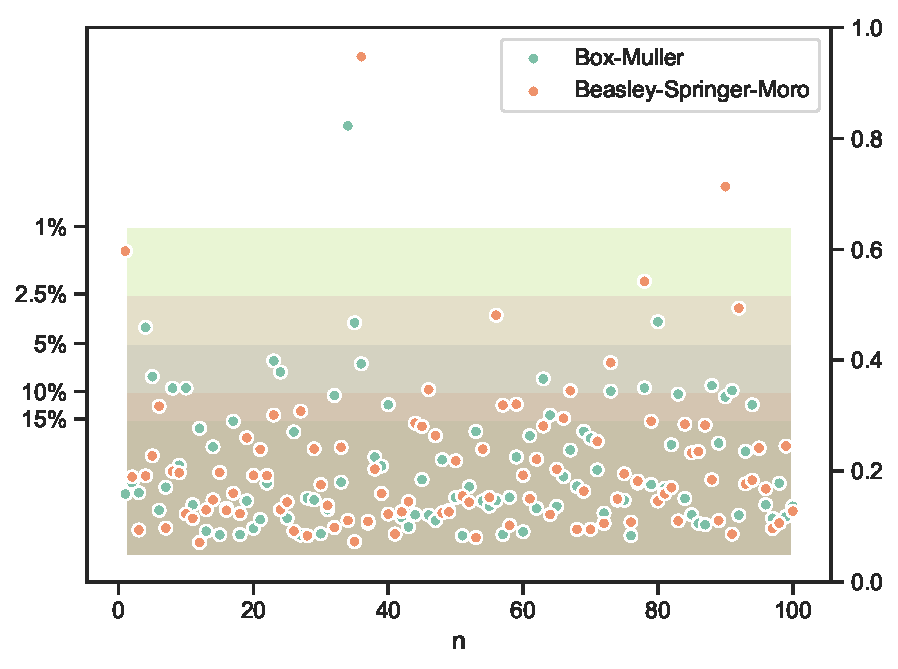
\includegraphics[scale=.95]{../figures/normality.pdf}
                    \label{fig:normality}
                \end{figure}

                As we can see in Table \ref{tab:normality}, the number of acceptances at significance level $k$ is approximately $100 - k$,
                which is what we would expect from normally-distributed data.
                However, the Beasley-Springer-Moro data set more closely matches the expected percentages than the Box-Muller data set does.
                This is most evident at the $15\%$ significance level, where the Box-Muller is giving only $79$ acceptances out of $100$
                instead of the expected $85$ out of $100$ that Beasley-Springer-Moro demonstrates.
                The data is visualized in Figure \ref{fig:normality}, where the significance levels are given by the shaded regions,
                and the plotted data is the Anderson-Darling statistic computed during each of the $100$ trials for each algorithm.

                Thus, we should conclude that the Beasley-Springer-Moro algorithm more faithfully simulates normally-distributed data than the Box-Muller algorithm.

        \end{enumerate}
    \item \label{5}
        {\it Consider a European call option with maturity $T = 1$, strike price $K = 50$, interest rate $r = 0.1$, volatility $\sigma = 0.3$, and initial price $S_0 = 50$.}
        \begin{enumerate}
            \item \label{5a}
                {\it Compute the Black-Scholes-Merton price of the option (i.e. the true price).}

                If we model the stock price as a Geometric Brownian Motion, we obtain the following general formula for the stock price assuming no arbitrage
                $S_t = S_0e^{\displaystyle\parens*{r - \sfrac{\sigma^2}{2}}t - \sigma W(t)}$
                where $W(t) \sim N\parens*{0, \sqrt{t}}$ is a standard Brownian motion.
                To find the price $C$ of a European call option written on $S$ with strike $K = 50$ with maturity $T = 1$,
                we use the Black-Scholes formula, here adapted from Baxter \& Rennie's Financial Calculus,
                \begin{align*}
                    C &= S_0\Phi\parens*{\frac{\log\parens*{\sfrac{S_0}{K}} + \parens*{r + \sfrac{\sigma^2}{2}}T}{\sigma\sqrt{T}}}
                    - Ke^{-rT}\Phi\parens*{\frac{\log\parens*{\sfrac{S_0}{K}} + \parens*{r - \sfrac{\sigma^2}{2}}T}{\sigma\sqrt{T}}}\\
                    &= 50\Phi\parens*{\frac{\log\parens*{1} + \parens*{0.1 + \sfrac{0.09}{2}}}{0.3}}
                    - 50e^{-0.1}\Phi\parens*{\frac{\log\parens*{1} + \parens*{0.1 - \sfrac{0.09}{2}}}{0.3}}\\
                    &= 50\parens*{\Phi\parens*{\frac{0.145}{0.3}} - e^{-0.1}\Phi\parens*{\frac{0.055}{0.3}}}\\
                    &\approx 50\parens*{0.6855704621388224 - e^{-0.1}0.5727317593030405}\\
                    &\approx 8.367066791193329,
                \end{align*}
                and approximated using Julia, where $\Phi$ is the standard normal cumulative distribution function.
            \item \label{5b}
                {\it Use random-shift Halton sequences with the Box-Muller method to obtain $40$ ``independent" estimates for the price of the option.
                For each estimate, use $N = 10,000$ price paths.}

                Random-shift Halton sequences of arbitrary dimension with prime bases were implemented in \texttt{task5.jl} file with the
                \texttt{halton(dim, len)} function, where \texttt{dim} is the dimension of the sequence and \texttt{len} is the number of
                \texttt{dim}-dimensional values to generate.
                We used $10$-dimensional Halton sequences as inputs for the $10$ time-step discretization of the Brownian motion.
                A $10$-dimensional sequence of length $10,000$ was used, with each $5$ number pair used as inputs to the Box-Muller method,
                and the $5$ normally-distributed output pairs used for simulating a different price path.
                The average expected value of the option was then computed by \texttt{priceBM()}.
            \item \label{5c}
                {\it Repeat part \ref{5b} using the Beasley-Springer-Moro algorithm.}

                Similarly to \ref{5b}, we use $10$-dimensional Halton sequences to generate normally-distributed values for the $10$ time steps of the Brownian motion.
                The price average price is computed by \texttt{priceBSM()}.
            \item \label{5d}
                {\it Compare the accuracy of the estimates computed in parts \ref{5b} and \ref{5c} as described in the assignment.}

                \begin{table}[H]
                    \centering
                    \caption{European Option Pricing with Halton Sequences}
                    \begin{tabular}{|r|c|c|c|c|c|c|c|c|} \hline
                                                & Mean              & Standard Deviation    & $A^2$       & 5\%    & 2.5\%  \\ \hline
                        Black-Scholes           & 8.367066791193329 & --                    & --          & --     & --     \\ \hline
                        Box-Muller              & 8.351529580745236 & 0.0450189795631       & 2.66411     & Reject & Accept \\ \hline
                        Beasley-Springer-Moro   & 8.37007120290087  & 0.0208181367092       & 0.59473     & Accept & Accept \\ \hline
                    \end{tabular}
                    \label{tab:price1}
                \end{table}

                The results of the $40$ trials are summarized in Table \ref{tab:price1} above, along with the results of the Anderson-Darling test.
                As we can see, both of the methods are very good estimators of the option price,
                but Box-Muller is rejected at the $5\%$ significance level while Beasley-Springer-Moro is accepted.
                In fact, Beasley-Springer-Moro is accepted even at the $10\%$ significance level.
                Therefore, we can reasonably conclude that the Beasley-Springer-Moro algorithm is better than the Box-Muller algorithm.
        \end{enumerate}
\end{enumerate}
\end{document}
